\documentclass{beamer}
\usetheme{Copenhagen}
\mode<presentation>

\usepackage{hyperref}
%\usepackage[francais]{babel}
%\usepackage[T1]{fontenc}
\usepackage[utf8]{inputenc}
\usepackage{beamerthemesplit}
\usepackage{graphicx}
\usepackage{caption}
\usepackage{subcaption}
\usepackage{listings}
\lstset{language=C}

% ------------- BODY ----------------

\title[From C loop nest to \texttt{multifor} loop nest]{Conversion of some well known polyhedral algorithms into his representation as a \texttt{multifor}
}

\author[Maxime Schmitt]{Maxime Schmitt \\ \scriptsize{maxime.schmitt@etu.unistra.fr}
}

\date{July 24, 2013}

\institute[ICube]{
    Department of Informatics \\
        ICube laboratories \\
        University of Strasbourg
}

\begin{document}

%---- titlepage ------

\begin{frame}
\titlepage{}

\tiny{
\begin{tabular}{|c|c|c|}
\hline
\bf{Philippe Clauss} & \bf{Imèn Fassi} & \bf{Eric Violard} \\
The multifor designer & Working on IBB & Working on the semantic \\
\hline
\end{tabular}
}
\centering{
    \begin{tabular}{cc}

    \begin{minipage}[t]{0.2\textwidth}
    
\includegraphics[width=\textwidth]{LOGOS/logoICube}
    \end{minipage}
    \begin{minipage}[t]{0.2\textwidth}
    
\includegraphics[width=\textwidth]{LOGOS/logo-uds-couleur-800433}
    \end{minipage}

    \end{tabular}
}
\end{frame}

%------- slide -------

\begin{frame}
\frametitle{Overview of the talk}
\tableofcontents{}
\end{frame}

%------- slide -------

\section{\texttt{Multifor}, what for?}

\subsection{The internship's goals}

\begin{frame}
\frametitle{What am I working on?}
\begin{itemize}

\item Conversion of the polyhedral benchmark into a \texttt{multifor} equivalence.
\item Find out what are the limitations.

\begin{itemize}

\item What does the semantics not allow?
\item Why can an algorithm be slower with the multifor than the sequential one?
\item Is it esay to take an existing algorithm and translate it into multifor?

\end{itemize}

\item Use IBB to convert multifor code to C source code and test it.

\end{itemize}
\end{frame}

%---------- frame -----------
\subsection{The \texttt{multifor} objectives}

\begin{frame}
\frametitle{Control/Task parallelism}

The \texttt{multifor} is based on control parallelism. \newline
Control parallelism consist on distributing sequential process across different parallel node, in oposition with data parallelism where you have a sequential code of parallel statements.

\begin{figure}[h]

\centering
\begin{minipage}[t]{0.30\textwidth}

\centering
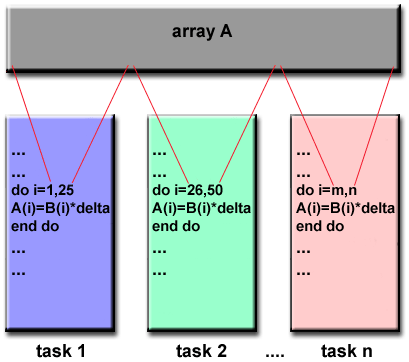
\includegraphics[width=\textwidth]{pictures/data-parallelism}
\centering{
Data parallelism
} \\
Example: MPI (Message passing interface)
\end{minipage}~% ------- "~"  add space between figure -> ~ \quad \qquad
\begin{minipage}[t]{0.30\textwidth}

\centering
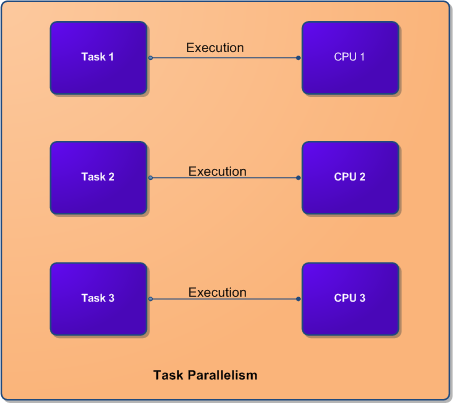
\includegraphics[width=\textwidth]{pictures/task-parallelism}
%\caption{Control parallelism}
\centering{
    Control parallelism
} \\
Example: HPF (High performance Fortran)
\end{minipage}

\end{figure}

\end{frame}

%--------------- frame ----------------

\begin{frame}
\frametitle{The aim of the \texttt{multifor}}

\begin{itemize}

\item In order to use more efficiently the resources of nowadays computers we have to work with appropriate tools.

\item The fact is that we already have lots of techniques to exhibit parallelism and optimize loops and wanted that not only compilers do that but programmers too.

\end{itemize}

\end{frame}

%-------------------- frame ----------------

\begin{frame}
\frametitle{Helping programmers}

\begin{itemize}

\item The programmer has only to worry about parallelizing and optimizing the code.
\item The \texttt{multifor} is only a control structure to simplify the implementation.
\item You can mix loop of different execution frequency and different starting point.

\end{itemize}

\end{frame}

%------------ frame ------------------

\begin{frame}
\frametitle{An incremental work}

The \texttt{multifor} will start by extending the C for structure. In the same way OpenMP is an extension to C/C++ and Fortran.\newline
In opposition we have the definition of new parallel languages like X10. \newline \newline
\begin{tabular}[l]{|p{0.48\textwidth}|p{0.48\textwidth}|}
\hline
\texttt{Multifor} & New parallel language \\
\hline
\color{green}{
    Is an extension of the well known for loop.\newline
    Can be implemented in existing languages.
}
&{
\color{green}{
Is implemented for parallel programming.
}
\color{red}{
\newline{}The programmer need to learn a new language and they often do not want.
}
}
\\
\hline
\end{tabular}

\end{frame}

%--------------- frame------------------

\subsection{Syntax and semantics reminding}

\begin{frame}
\frametitle{Syntax}

\small{ $\begin{array}{l}
    \bf{multifor}(int~{\color{red}i_0{=}0}, {\color{blue}i_1{=}0};
            {\color{red}i_0{<}6}, {\color{blue}i_1{<}3};
            {\color{red}i_0}++, {\color{blue}i_1}++;
            {\color{red}1}, {\color{blue}2};
            {\color{red}0}, {\color{blue}1})\{
    \\
        \quad{}\bf{multifor}(int~{\color{red}j_0{=}0}, {\color{blue}j_1{=}0};
                {\color{red}j_0{<}6}, {\color{blue}j_1{<}3};
                {\color{red}j_0}++, {\color{blue}j_1}++;
                {\color{red}1}, {\color{blue}2};
                {\color{red}0}, {\color{blue}2})\{
    \\
        \qquad{}{\color{red}0:\{ statement[i_0][j_0]\ldots \}}
    \\
        \qquad{}{\color{blue}1:\{ statement[i_1][j_1]\ldots \}}
    \\
        \quad{}\}
\\
    \}
\end{array}$
}

\centering{
    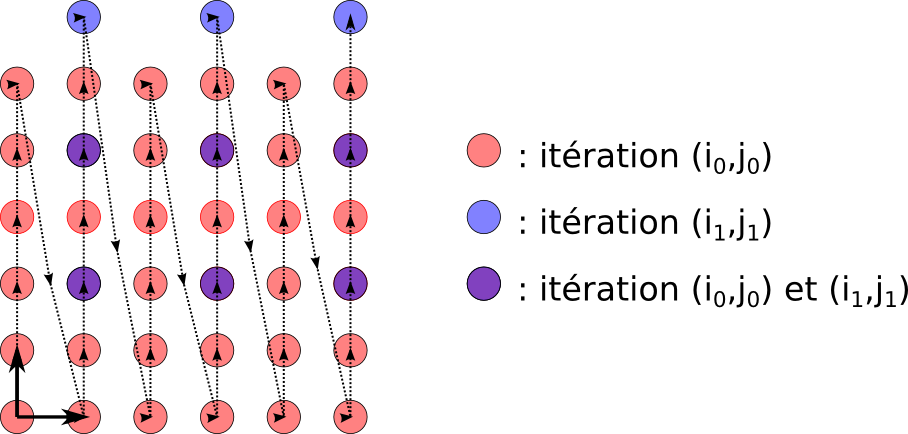
\includegraphics[height=3.5cm]{pictures/referential_domain}
}

\end{frame}

%-------------- frame -------------------

\section{From for to \texttt{mulifor}}
\subsection{Eric's approach}

\begin{frame}
\frametitle{Game of life}

Rules:
\begin{itemize}
\item If a cell has exactly 3 neighbours it live the next time step.
\item If a cell has exactly 2 neighbours it states is unchanged.
\item Otherwise the cell dies.
\end{itemize}

\end{frame}

%------------- frame -------------

\begin{frame}
\frametitle{The game of life algorithm}

{$\begin{array}{l}

    int~t[N][N]; \\
        int~temp[N-2][N-2]; \\ \\
        \textbf{void} calc ()\{ \\
        ~\textbf{{\color{red}for}}~(int~i=1; i<N-1; i++) \\
        \quad{}\textbf{{\color{red}for}}~(int~j=1; j<N-1; j++)\{ \\
        \qquad{}temp[{\color{green}i-1}][{\color{green}j-1}]=\\
        \qquad{}game\_of\_life(t[{\color{cyan}i}][{\color{cyan}j}],t[{\color{cyan}i-1}][{\color{cyan}j}],t[{\color{cyan}i-1}][{\color{cyan}j-1}],t[{\color{cyan}i-1}][{\color{cyan}j+1}],\\
                \qquad{}[{\color{cyan}i}][{\color{cyan}j-1}],[{\color{cyan}i}][{\color{cyan}j+1}],[{\color{cyan}i+1}][{\color{cyan}j-1}],[{\color{cyan}i+1}][{\color{cyan}j}],[{\color{cyan}i+1}][{\color{cyan}j+1}]); \\
        \quad{}\}\\
        ~\textbf{{\color{blue}for}}~(int~i=1; i<N-1; i++) \\
        \quad{}\textbf{{\color{blue}for}}~(int~j=1; j<N-1; j++)\{ \\
        \qquad{}t[i][j]=temp[i-1][j-1]; \\
        \quad{}\} \\
        \}



\end{array}$
}

\end{frame}

%---------- frame -------------

\begin{frame}
\frametitle{The game of life iteration domain}

\centering{
\includegraphics{pictures/gameoflife}
}

\end{frame}

%------------------- frame -------------------

\begin{frame}
\frametitle{The same algorithm as \texttt{mulifor}}

{$\begin{array}{l}

    void~calc\_multifor ()\{ \\
        ~multifor({\color{red}i=1}, {\color{blue}i2=1}; {\color{red}i<N-1}, {\color{blue}i2<N-1}; {\color{red}i++}, {\color{blue}i2++};{\color{red} 1}, {\color{blue}1}; {\color{red}0}, {\color{blue}3})\{ \\
            \quad{}multifor({\color{red}j=1}, {\color{blue}j2=1}; {\color{red}j<N-1}, {\color{blue}j2<N-1}; {\color{red}j++}, {\color{blue}j2++}; {\color{red}1}, {\color{blue}1}; {\color{red}0}, {\color{blue}0})\{ \\
\qquad{}0:\{\\
\qquad{}~~temp[i-1][j-1]= \\
\qquad{}~~game\_of\_life(t[i][j],t[i-1][j],t[i-1][j-1],t[i-1][j+1], \\
\qquad{}~~[i][j-1],[i][j+1],[i+1][j-1],[i+1][j],[i+1][j+1]); \\
\qquad{}\} \\
\qquad{}1:  t[i2][j2]=temp[i2-1][j2-1]; \\
           \quad{}\} \\
        ~\} \\
    \} \\


    \end{array}$
}

\end{frame}

\end{document}
